\documentclass{sigchi}

% Use this command to override the default ACM copyright statement
% (e.g. for preprints).  Consult the conference website for the
% camera-ready copyright statement.

%% EXAMPLE BEGIN -- HOW TO OVERRIDE THE DEFAULT COPYRIGHT STRIP -- (July 22, 2013 - Paul Baumann)
% \toappear{Permission to make digital or hard copies of all or part of this work for personal or classroom use is      granted without fee provided that copies are not made or distributed for profit or commercial advantage and that copies bear this notice and the full citation on the first page. Copyrights for components of this work owned by others than ACM must be honored. Abstracting with credit is permitted. To copy otherwise, or republish, to post on servers or to redistribute to lists, requires prior specific permission and/or a fee. Request permissions from permissions@acm.org. \\
% {\emph{CHI'14}}, April 26--May 1, 2014, Toronto, Canada. \\
% Copyright \copyright~2014 ACM ISBN/14/04...\$15.00. \\
% DOI string from ACM form confirmation}
%% EXAMPLE END -- HOW TO OVERRIDE THE DEFAULT COPYRIGHT STRIP -- (July 22, 2013 - Paul Baumann)
\toappear{}

% Arabic page numbers for submission.  Remove this line to eliminate
% page numbers for the camera ready copy
% \pagenumbering{arabic}

% Load basic packages
\usepackage{balance}  % to better equalize the last page
\usepackage{graphics} % for EPS, load graphicx instead 
\usepackage[T1]{fontenc}
\usepackage{txfonts}
\usepackage{mathptmx}
\usepackage[pdftex]{hyperref}
\usepackage{color}
\usepackage{booktabs}
\usepackage{textcomp}
% Some optional stuff you might like/need.
\usepackage{microtype} % Improved Tracking and Kerning
% \usepackage[all]{hypcap}  % Fixes bug in hyperref caption linking
\usepackage{ccicons}  % Cite your images correctly!
% \usepackage[utf8]{inputenc} % for a UTF8 editor only

% If you want to use todo notes, marginpars etc. during creation of your draft document, you
% have to enable the "chi_draft" option for the document class. To do this, change the very first
% line to: "\documentclass[chi_draft]{sigchi}". You can then place todo notes by using the "\todo{...}"
% command. Make sure to disable the draft option again before submitting your final document.
\usepackage{todonotes}
\usepackage[frenchb]{babel}
%\frenchbsetup{og = �, fg = �}

% Paper metadata (use plain text, for PDF inclusion and later
% re-using, if desired).  Use \emtpyauthor when submitting for review
% so you remain anonymous.

%----------------------------------------------------------------------------------------
% Title, Authors, Keywords
%----------------------------------------------------------------------------------------
\def\plaintitle{GraspMe: A Grasp Sensitive Adaptive Slider for Mobile Devices}
\def\plainauthor{First Author, Second Author, Third Author,
  Fourth Author, Fifth Author, Sixth Author}
\def\emptyauthor{}
\def\englishkeywords{Authors' choice; of terms; separated; by
  semicolons; include commas, within terms only; required.}
\def\frenchkeywords{Format ; instructions ; qualit\'{e} ; actes de conf\'{e}rence ; les mots cl\'{e}s doivent \^{e}tre s\'{e}par\'{e}s par des point-virgules.}
\def\plaingeneralterms{Documentation, Standardization}
%----------------------------------------------------------------------------------------

% llt: Define a global style for URLs, rather that the default one
\makeatletter
\def\url@leostyle{%
  \@ifundefined{selectfont}{
    \def\UrlFont{\sf}
  }{
    \def\UrlFont{\small\bf\ttfamily}
  }}
\makeatother
\urlstyle{leo}

% To make various LaTeX processors do the right thing with page size.
\def\pprw{8.5in}
\def\pprh{11in}
\special{papersize=\pprw,\pprh}
\setlength{\paperwidth}{\pprw}
\setlength{\paperheight}{\pprh}
\setlength{\pdfpagewidth}{\pprw}
\setlength{\pdfpageheight}{\pprh}

% Make sure hyperref comes last of your loaded packages, to give it a
% fighting chance of not being over-written, since its job is to
% redefine many LaTeX commands.
\definecolor{linkColor}{RGB}{6,125,233}
\hypersetup{%
  pdftitle={\plaintitle},
% Use \plainauthor for final version.
%  pdfauthor={\plainauthor},
  pdfauthor={\emptyauthor},
  pdfkeywords={\englishkeywords},
  bookmarksnumbered,
  pdfstartview={FitH},
  colorlinks,
  citecolor=black,
  filecolor=black,
  linkcolor=black,
  urlcolor=linkColor,
  breaklinks=true,
}

% create a shortcut to typeset table headings
% \newcommand\tabhead[1]{\small\textbf{#1}}

% End of preamble. Here it comes the document.
%----------------------------------------------------------------------------------------
\begin{document}

\title{\plaintitle}

\numberofauthors{3}
\author{%
  \alignauthor{Premier Auteur\\
    \affaddr{Affiliation}\\
    \affaddr{Code postal, Ville, Pays}\\
    \email{Adresse email}}\\
  \alignauthor{Deuxi\`{e}me Auteur\\
    \affaddr{Affiliation}\\
    \affaddr{Code postal, Ville, Pays}\\
    \email{Adresse email}}\\
  \alignauthor{Troisi\`{e}me Auteur\\
    \affaddr{Affiliation}\\
    \affaddr{Code postal, Ville, Pays}\\
    \email{Adresse email}}\\
}

%================================================
%\begin{figure*}[h]
%  \centering
%  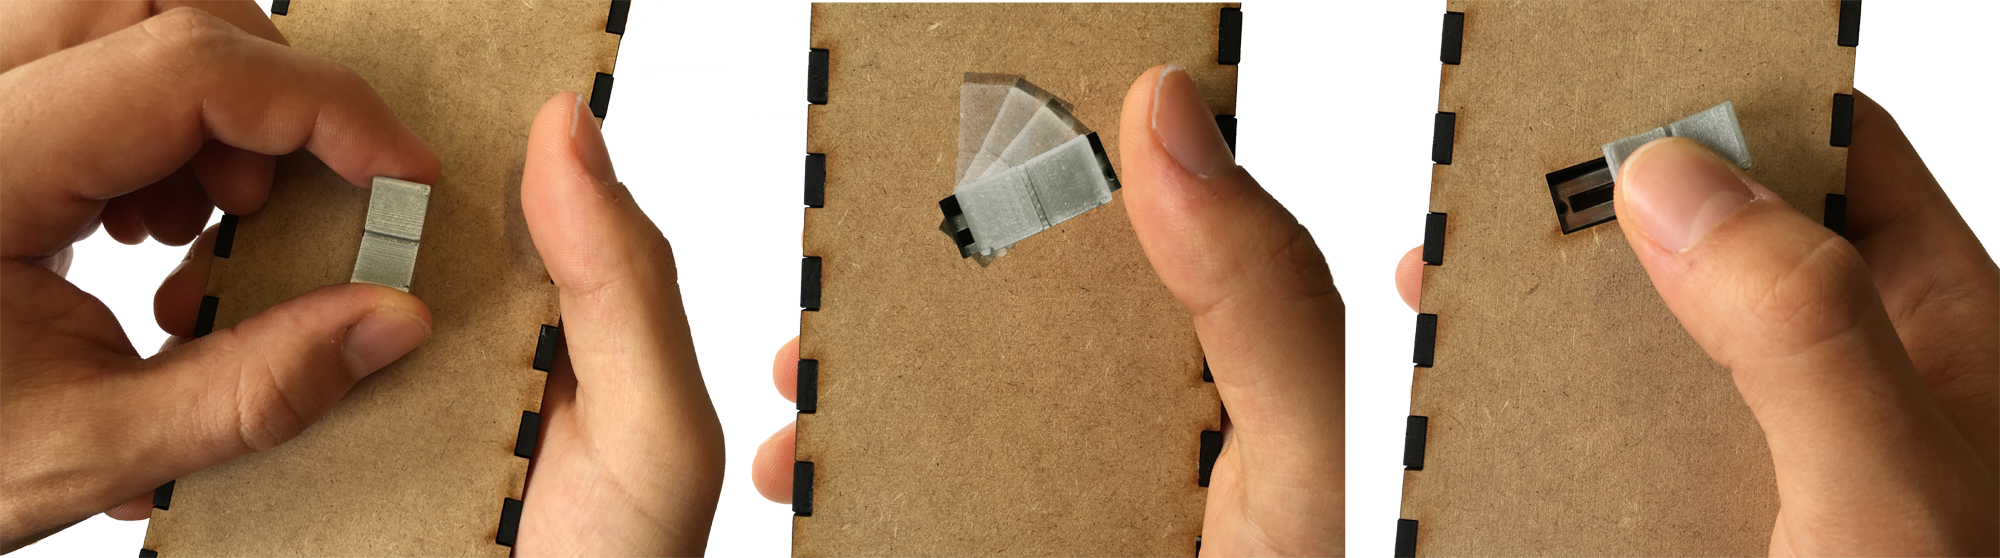
\includegraphics[width=1.7\columnwidth]{figures/portada}
%  \caption{GraspMe concept: the slider changes size and orientation according to the way how it is operated}
%\end{figure*}
%================================================ 

\makeatletter
\let\@oldmaketitle\@maketitle% Store \@maketitle
\renewcommand{\@maketitle}{\@oldmaketitle% Update \@maketitle to insert...
  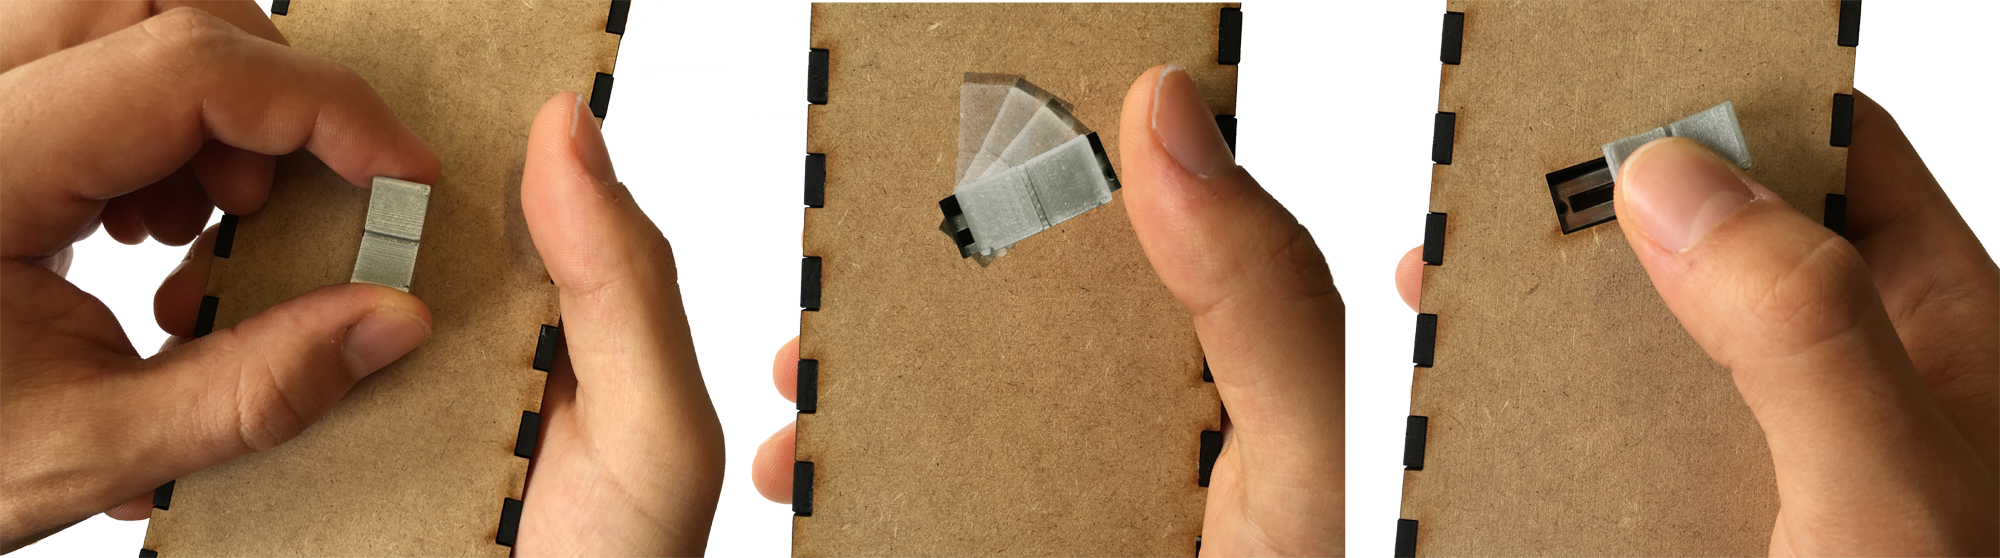
\includegraphics[width=\linewidth,height=5\baselineskip]
    {figures/portada}\bigskip}% ... an image
\makeatother

\maketitle


%----------------------------------------------------------------------------------------
\begin{resume} % R�sum�
%----------------------------------------------------------------------------------------
	MAJ---\today. Cet article d\'{e}crit et utilise le format de mise en page \`{a} respecter pour les soumissions \`{a} IHM'16. Apr\`{e}s acceptation, ces soumissions seront publi\'{e}es dans les actes d'IHM'16, ainsi que sur l'ACM Digital Library, sauf les communications informelles qui seront publi\'{e}es dans un volume annexe s\'{e}par\'{e}. Comme certains \'el\'ements ont chang\'{e} par rapport aux ann\'{e}es pr\'{e}c\'{e}dentes, nous vous prions de bien lire ce document m\^{e}me si vous avez d\'{e}j\`{a} soumis \`{a} IHM auparavant.
\end{resume}

\motscles{\frenchkeywords} %Mots cl�s
%----------------------------------------------------------------------------------------

%----------------------------------------------------------------------------------------
\begin{abstract} % English Abstract (mandatory)
%----------------------------------------------------------------------------------------
  UPDATED---\today. This article describes the formatting requirements for IHM'16. After acceptance, these submissions will be published in the proceedings of IHM'16 and the ACM Digital Library. As some items have changed from previous years, please read the document carefully, even if you have submitted to IHM before. Please add an additional abstract in English, along with the French version.
\end{abstract}

\keywords{\englishkeywords} % English keywords (mandatory)
%----------------------------------------------------------------------------------------

%----------------------------------------------------------------------------------------
\category{H.5.m.}{Information Interfaces and Presentation
  (e.g. HCI)}{Miscellaneous} \category{See
  \url{http://acm.org/about/class/1998/} for the full list of ACM
  classifiers. This section is required.}{}{}
%----------------------------------------------------------------------------------------

%----------------------------------------------------------------------------------------
\section{Introduction}
%----------------------------------------------------------------------------------------
Le format d\'{e}crit dans ce document doit \^{e}tre respect\'{e} pour les soumissions \`{a} la conf\'{e}rence IHM. Nous souhaitons faire des actes d'IHM un document de qualit\'{e} \`{a} la pr\'{e}sentation homog\`{e}ne. Nous demandons donc aux auteurs de respecter quelques r\`{e}gles simples. 

Nous vous demandons principalement de faire en sorte que votre article ressemble exactement \`{a} ce document. La meilleure fa\c{c}on d'y parvenir est de t\'{e}l\'{e}charger l'un des mod\`{e}les propos\'{e}s depuis le site web de la conf\'{e}rence IHM, \url{http://ihm16.afihm.org/#!contribution}, et de remplacer son contenu par le v\^otre.

%----------------------------------------------------------------------------------------
\section{Motivation}
%----------------------------------------------------------------------------------------
We have identified three main aspects as the motivation of our work: the different ways users hold their mobile devices, the different ways a slider can be operated, and the relevance of sliders on mobile devices. Regarding the ways users interact with their mobile devices, the literature exposes two main reasons for changing hands’ position: internal limitations and external limitations of the mobile device. Before detailing these limitations we present works related to the variability of mobile interaction.

%----------------------------------------------------------------------------------------
\subsection{A large diversity in the grasp of mobile devices}
%----------------------------------------------------------------------------------------
In \cite{Karlson06} a survey was presented in which participants were asked how many hands do they use to perform typical mobile tasks and the numbers of hands they would prefer to use. 45\% stated they use one hand for almost all mobile interactions and only 19\% stated the same for two hands. Related to the preference 66\% stated they would prefer using just one hand for the tasks and only 9\% would prefer using both hands.

An observational study \cite{hoober13} showed that from 780 persons there are three basic ways in which users hold their mobile phones while interacting with it\footnote{Values are approximations, no absolute value was obtained.}: 49\% interacted with the same hand that holds the phone, 36\% interacted with one hand while holding the device with the other hand and 15\% interacted with both hands. In the study they also observed that people change the way they hold their device quite often (in some cases every few seconds) and the grasps are not static states. Though the work did not study this in depth, the author argues (through observation of users interacting with their device) that the main reason for this is related to the task the user is performing (e.g. one hand grasp for swiping, two hands grasp for tapping).

Nowadays most portable devices have a touchscreen as the main input entry, leading users to make use of gestures and taps to interact with the device. Gestures such as swiping make use of just one digit (usually thumb or index finger), pinching gestures make use of two digits (index-thumb for one hand or thumb-thumb for both hands) and some gestures like double tapping can be performed with one or two digits at the same time. These gestures are used widely on portable devices to activate functionalities: zooming in and out can be achieved with a pinching or double tap gesture, sliding is typically used for scrolling through text and single tapping for target selection. We can think of an user that types in a web address, scrolls down through its content and zoom in certain area to read better; for this, several gestures must be performed and hence, different grasps.

But gestures are internal limitations of the device, external limitations (e.g. encumbrance) can also alter the way users grasp their devices. Indeed, the fact of being mobile allow users to move and thus, be able to perform other activities such as shopping, cooking, walking, etc., in which user can be sensory restricted (looking the street while crossing it) or articulatory restricted (carrying heavy objects).
 
Encumbrance effect on mobile interaction has been studied \cite{NgA11,Ng2013,Ng:2013:REW:2468356.2468599,Mainwaring2005}. In \cite{Ng:2014:IEE:2556288.2557312} the effect of encumbrance on one- and two-handed interaction for mobile devices was studied. Three basic input grasps (Figure ~\ref{fig:figure1}) were evaluated: two-handed index finger, one-handed preferred thumb and two-handed both thumbs. A target selection task experiment was performed with these input grasps while the user was encumbered with plastic bags (in one and in both hands) and in motion. Results show a decrease in performance when users are in motion and one-handed encumbered (17\% error rate) and also when in motion and two-handed encumbered (10\% error rate).

%================================================
\begin{figure}[h]
\centering
  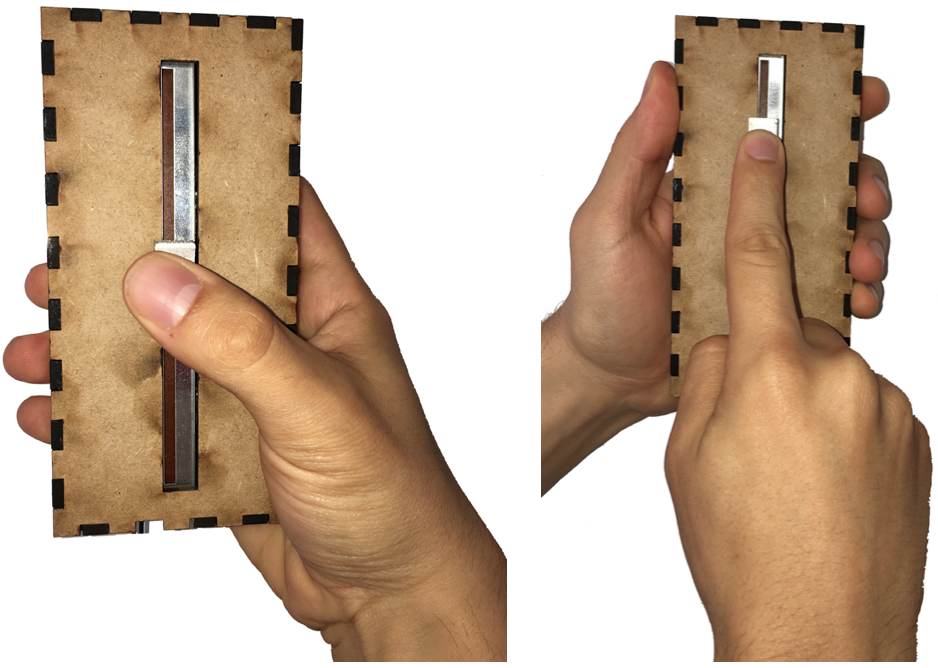
\includegraphics[scale=0.3]{figures/1}
  \caption{}
  \label{fig:figure1}
\end{figure}
%================================================

%----------------------------------------------------------------------------------------
\subsection{Benefit of Tangible Sliders for Mobile Devices}
%----------------------------------------------------------------------------------------
Mobile devices let us interact with applications or appliances in a discrete or continuous manner. Digital sliders have been used to control a wide diversity of functions (e.g. a device’s screen brightness or volume) and appliances such as mixing consoles and smart house’s control panel at distance. Though digital sliders offer flexibility of arrangement in the screen, certain features are lost with graphical widgets which can be achieved with tangible sliders, such as eyes-free interaction.

The benefits of tangible elements are well known in the HCI community. Regarding tangible sliders, in \cite{Jansen:2012:TRC:2207676.2208691} tangible sliders, which could be placed on top of a tablet’s screen, were used to control wall-size displays. The advantages of the tangible and mobile interaction let participants of the study control an appliance at distance while carrying the portable device and being eyes-free from the device. The usefulness of merging both interaction techniques was also examined in \cite{unpublished}, in which a similar study was carried with sliders and knobs. Participants were also able to control a distant appliance and were able to move (spin) while operating the device.

%----------------------------------------------------------------------------------------
\subsection{A large diversity in the grasp of tangible sliders}
%----------------------------------------------------------------------------------------
Tangible continuous controls such as tangible sliders have been studied for a long time \cite{Kroemer}. Indeed, these widgets have been useful to control continuous parameters; we can find them in mixing boards, cars, smart houses’ control panel and even in military facilities and aircrafts. 
In \cite{standrs} a standardisation of the factors such as visual and tactile examination are presented in relation to how users interact with a slider. Authors present several sliders’ knob shapes and how user can interact with them; two main interaction techniques are presented: normal pinching (Figure ~\ref{fig:figure2}, row a) and tangential contact (Figure ~\ref{fig:figure2}, row b).

%================================================
\begin{figure}[h]
\centering
  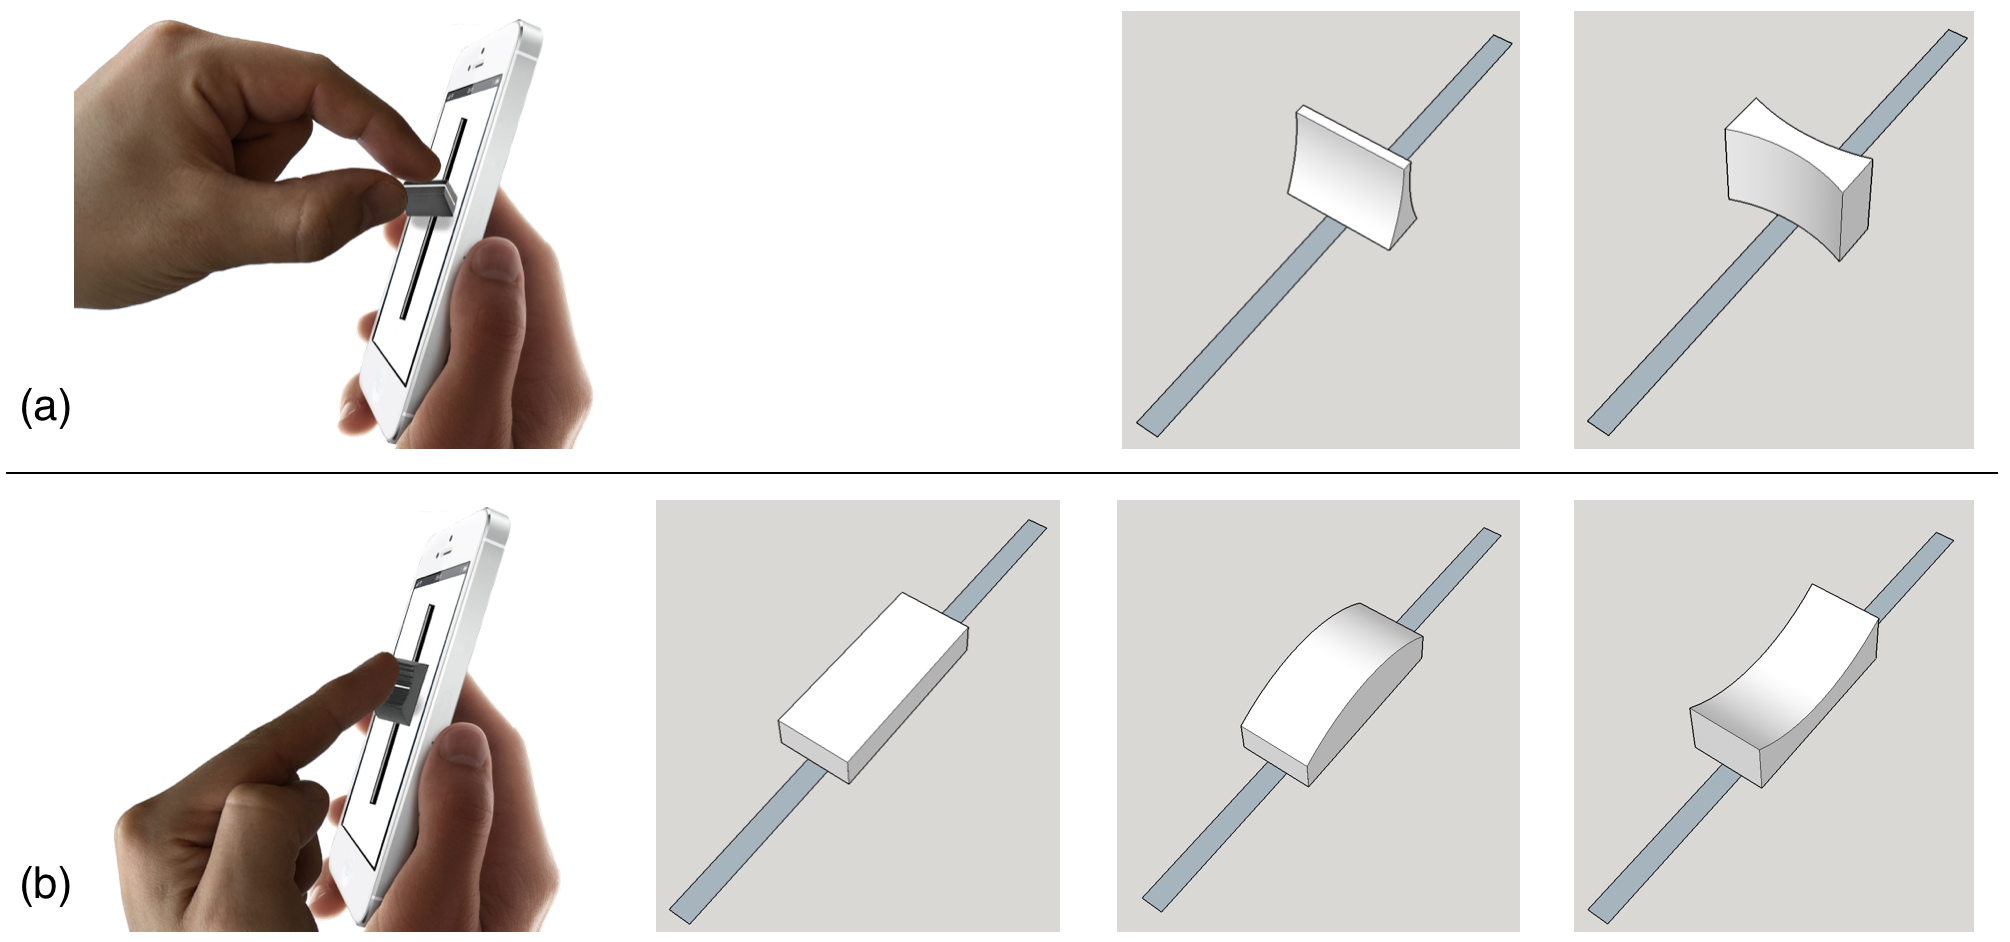
\includegraphics[width=0.9\columnwidth]{figures/2}
  \caption{}
  \label{fig:figure2}
\end{figure}
%================================================

After reviewing these main aspects, we can notice the importance of tangible controls such as a slider on portable devices and a clear need of adapting this widget to the grasp the user performs. Deformable portable devices \cite{unpublished,Hemmert:2008:DKS:1358628.1358675,Roudaut:2013:MTH:2470654.2470738,Dimitriadis:2014:EEP:2556288.2557164} serve as inspiration in this work to propose a deformable slider for mobile devices; the following scenario illustrates the usability of such apparatus.

%----------------------------------------------------------------------------------------
\section{Case Scenario: Smarthouse Control}
%----------------------------------------------------------------------------------------
Alice is in the supermarket paying some products she bought for a romantic dinner she is planning tonight. While she waits for the cashier to finish the payment, she starts her deformable smartphone. While grabbing the device with one hand, with the other hand she starts adjusting the temperature in her house by moving a tangible vertical slider, nearly of the size of the screen, that deformed in the screen of her smartphone. Alice gets interrupted by the cashier who has finished the payment and due to the people waiting in queue she decides to take her bags and continuing adjusting the temperature with one hand while going back home; for this, the slider widget deforms and changes to a tilted orientation and a smaller size in order to facilitate thumb interaction. At home, Alice receives a call on her fixed phone; while talking on the phone she controls the TV with her smartphone and forwards a cuisine episode about a dessert she wants to prepare. Her phone call ends and she takes the deformable smartphone with both hands to precisely adjust the frame to the moment when the dessert explanation starts. Now Alice is prepared for a romantic night with some gourmet dessert.

%----------------------------------------------------------------------------------------
\section{Related Work}
%----------------------------------------------------------------------------------------

%----------------------------------------------------------------------------------------
\subsection{Deformable Tangible User Interfaces}
%----------------------------------------------------------------------------------------
In \cite{Murakami:1995:DDO:223355.223442}, a deformable object is used as a tool to manipulate and deform its virtual 3D representation. This early work studied the benefits of deformable tangible objects as an interface through a general shape (a cube); we will focus specifically on sliders.

In \cite{Michelitsch:2004:HCN:985921.986050}, a deformable widget knob is presented; the user can change the form of the knob for a thinner one to operate a video playback in frame-by-frame mode and by using a round shape of the knob the user operates in scene-by-scene mode. In this approach users perform always the same type of grasp on the widget, we want to focus in the deformation of widgets when the grasp changes (e.g. one digit contact to two digits grip). On top of that, the deformation of the widget produces a change in the task; in this work we will focus on different grasps while performing the same task.

On both works a lack of mobility is present, our work is focused on the domain of portable devices and thus, mobile.

%----------------------------------------------------------------------------------------
\subsection{Mobile Deformable Tangible User Interfaces}
%----------------------------------------------------------------------------------------
Going into the portable field, in \cite{Hemmert:2008:DKS:1358628.1358675} authors explored the use of tangible elements on mobile devices to give feedback about phone-like events (calls, messages, alarms, etc.). In \cite{Roudaut:2013:MTH:2470654.2470738,Dimitriadis:2014:EEP:2556288.2557164} a shape-changing portable device deforms itself to give tactile feedback to the user. In \cite{Hardy:2015:STR:2702123.2702599} a set of linear actuators were used on top of a capacitive screen to act as a z-actuating widget. In all these cases, the benefit of deformable interfaces lied in the output.

We are aiming to use tangibility as an input channel. In \cite{Jansen:2012:TRC:2207676.2208691} tangible sliders were used on top of a tablet screen in order to control a wall-size display application. In \cite{unpublished} deformable portable devices for controlling continuous parameters were analysed; authors presented a high-resolution prototype (with real tangible controls) and a low-resolution prototype (a pixel-based approach) with sliders and dials as controls. The prototypes’ system was able to deform the interface according to a task. On both works tangibility is used as an input channel but the deformation aspect was achieve in different ways: in \cite{Jansen:2012:TRC:2207676.2208691} by bringing a digital slider to a physical one and in \cite{unpublished} by changing a slider for a knob. In this work we will tackle the deformation aspect by changing physical attributes of the slider (e.g. change the orientation of the slider).

%----------------------------------------------------------------------------------------
\subsection{Adaptation for One- and Two- Hands Interaction}
%----------------------------------------------------------------------------------------
Due to the changing grasp of portable devices, researchers and designers have focused on adapting the interfaces according to the type of interaction performed by the user (one or two handed). In \cite{Taylor:2009:GGU:1518701.1518842}, authors proposed to detect the grip on a tangible object and adapt the action performed accordingly to the application it interacts with (e.g. turning a digital Rubik’s cube). The work focused on adapting graphical objects on a distant screen; we will focus on deforming controls placed on the top surface of the portable device.

The way we grasp a portable device usually leaves our fingers (with exception of the thumb) on the backside of the device \cite{hoober13}. Taking this into account, several works proposed backside interaction \cite{Baudisch:2009:BIA:1518701.1518995,Wigdor:2007:LTS:1294211.1294259}. With iRotateGrasp \cite{Cheng:2012:IGA:2380296.2380305}, the orientation of a mobile UI (landscape or portrait) follows the users grasp on the device instead of the absolute orientation that follows the earth gravity. This allows, for example, landscape-oriented UI while lying on a bed; however adaptation is graphical only. We focus on adaptation of tangible user interfaces.  

In \cite{Cheng:2013:IGA:2468356.2479514}, the authors propose an adaptive keyboard that takes into consideration grasping style and functional surface to offer a graphical keyboard at optimal locations. In \cite{Wagner:2012:BBD:2207676.2208391}, sensors on a tablet are able to recognise the grasping style and offers new functionalities to be operated with the non-dominant hand. These examples present how the grasp can be use in the input channel. Nevertheless it is centred for discrete functions, we want to explore continuous parameters. They also lack the tangibility that is beneficial for interaction \cite{unpublished,Jansen:2012:TRC:2207676.2208691}.  

In \cite{Negulescu:2015:GCI:2702123.2702185} the changes (tilt and shift) of the grasp of a mobile phone when the user tries the maximum reach of the current hand posture was analysed. Authors presented a model that predicts the intended user’s touchdown (area in which the finger will land) when interacting with the device’s screen. The model makes predictions of the finger’s touchdown while it is still en-route, aiming to adjust the actual input to the intended target.

A challenge related to interaction with hand-held touchscreen is the incapacity of users to reach the entire surface with the thumb of the hand that holds the device. As technology advances, screens get larger and our hands smaller in comparison. The area that can be reached with the thumb is called functional area of the thumb and designers have long been aware of this problem. Several heuristics have been proposed \cite{hoober13,Clark,Curtis,Wroblewski} to serve as reference but these are just rough estimations. In \cite{Bergstrom-Lehtovirta:2014:MFA:2611528.2557354} a model to estimate the functional area of the thumb through grip related information is presented. The model outputs the functional area that is commonly an area under a parabolic curve; similar areas are represented in the heuristic approaches. Following the flow of these works, we want to adapt tangible user interfaces according to the way users hold their portable devices.

Current tangible slider knobs are meant to be operated with a pinch grip or with one digit contact in a tangential way \cite{standrs}. Thinking about using a thumb to operate a tangible slider might seem bizarre, specially considering that the thumb makes a parabolic movement in comparison with the linear movement a slider requires. Considering the fact that there is no current slider knob tailored for thumb interaction, we propose the use of a slider composed of a concave knob for thumb positioning and with a tilted orientation instead of a vertical one, which fits better under the functional area of the thumb.

%----------------------------------------------------------------------------------------
\section{Preliminary Study}
%----------------------------------------------------------------------------------------
We conducted an experiment to evaluate the impact of grasping on the performance with different tangible sliders on a mobile device for a pointing task. The experiment followed a within-subjects design with three independent variables:

\begin{itemize}
\item \textbf{Length:} Small, large
\item \textbf{Orientation:} Vertical, tilted
\item \textbf{Interaction Technique:} One- or two-handed
\end{itemize}

The Length variable refers to the travel length of the slider’s knob, the values are: 20mm length and 70mm length. The Orientation variable is composed of two states: vertical (90 degrees) and tilted (68 degrees). The Interaction Technique variable represents the way how the mobile device is operated: one-handed, for thumb interaction, and two-handed, for using one hand to hold the devices and interacting with the second hand.
%----------------------------------------------------------------------------------------
\subsection{Apparatus}
%----------------------------------------------------------------------------------------
To measure the need of a deformable portable device, we built four prototypes (Figure \ref{fig:prototypes}) to analyse their performance when operated with one or two hands: two versions of a commonly used vertical-oriented slider and two versions with a tilted orientation. Versions varied in the sliding range of the slider. For both the vertical oriented and tilted oriented prototypes, a 20mm and a 70mm sliding range slider versions were built. Commercial sliders widgets vary in length from 20mm to 100mm \cite{Coutrix2015}; in \cite{Hirotaka:2003:RCC:765891.766081} the movement range of the thumb was analysed and authors stated an average thumb’s length of 60.4mm and an average rotation angle of 68.1 degrees, which was used as the angle on the tilted oriented version. By calculating the chord (Equation 1) between the points of the thumb’s rotation angle we obtained (in average) the longest straight line that the thumb can perform, this is 70.16mm; where: \textit{r} is the radius, in this case the thumb’s length; and $\theta$ is the angle subtended by the chord, in this case the thumb’s rotation angle.

%================================================
\begin{equation}
D=2r\sin\Big(\frac{\theta}{2}\Big)
\end{equation}
%================================================

The slider knob of the prototypes have a concave shape in order to allow one-digit operation with the thumb only and also two-digit operation when holding the device with one hand and interacting with the second one (Figure \ref{fig:figure3}); we have chosen this design to facilitate both grasps. All prototypes were built following the dimensions of a modern smartphone\footnote{iPhone 6s: http://www.apple.com/iphone-6s/specs/} in order to keep the grasping of the device as close to real portable devices. Prototypes were built using 3mm-thick wood (Medium-density fibreboard). As sliders, we used the following Bourns models\footnote{http://www.bourns.com/products/potentiometers/slide-potentiometers}: PTA2043-2015CPB103 (20mm sliding range) and PTB0143-2010BPB103 (100mm sliding range, cut up to 70mm).

%================================================
\begin{figure}[h]
\centering
  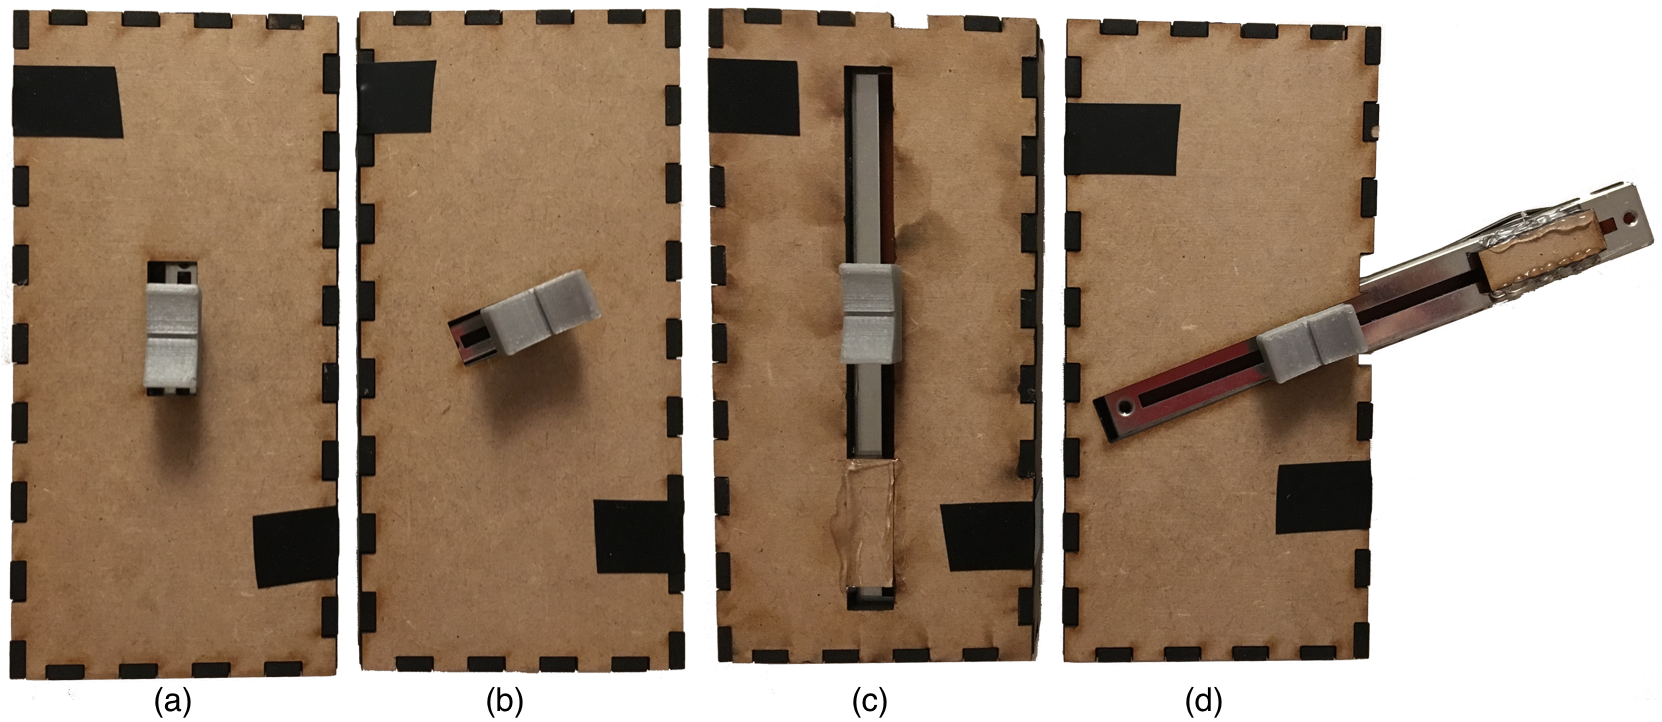
\includegraphics[width=1\columnwidth]{figures/prototypes}
  \caption{}
  \label{fig:prototypes}
\end{figure}
%================================================

%================================================
\begin{figure}[h]
\centering
  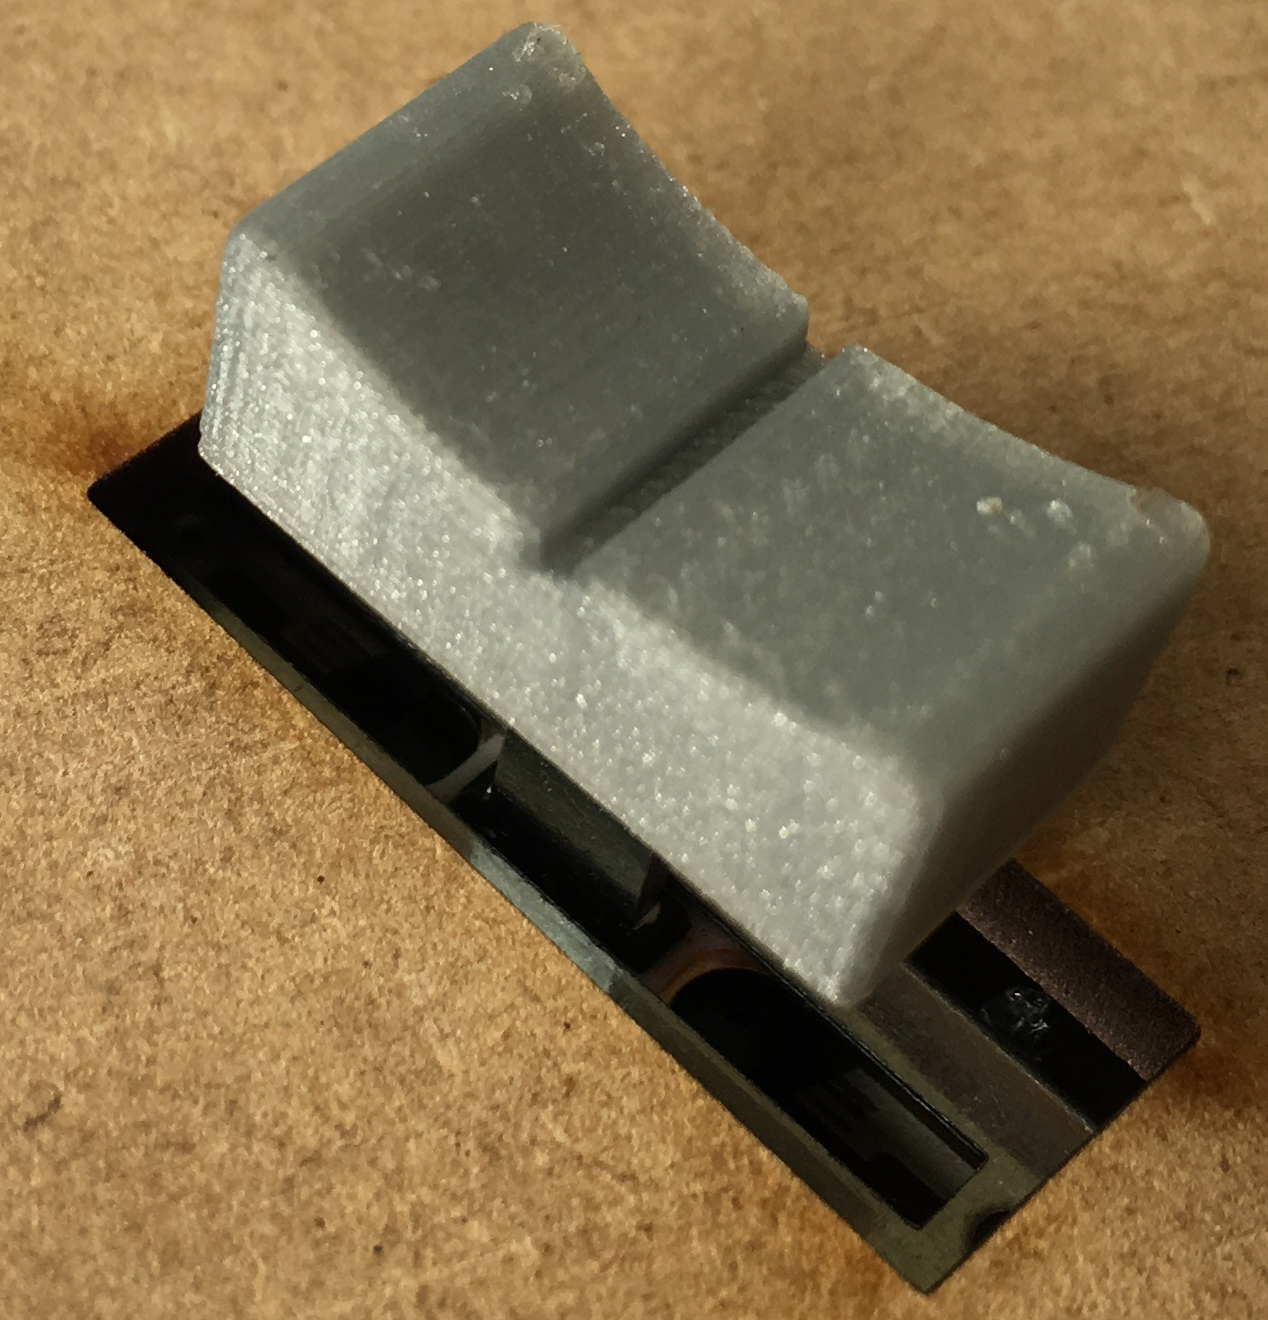
\includegraphics[width=0.4\columnwidth]{figures/knob}
  \caption{}
  \label{fig:figure3}
\end{figure}
%================================================

The four prototypes were connected to an Arduino Mega 2560 board in order to make the connection with our pointing task software. We made use of a 15 inches MacPro screen with 220 pixels per inch (ppi) to display the task.

%----------------------------------------------------------------------------------------
\subsection{Task}
%----------------------------------------------------------------------------------------
The preliminary study required participants to perform a pointing task as in previous work \cite{Buck:Motor}. We have chosen this type of task to evaluate the performance of the prototypes under different grasping techniques. The task consist of positioning a cursor (controlled by the user) inside a target area on top of a thin vertical white slider of 75mm/331px. Following the case scenario, the target area has a width of 4mm/16px in order to resemble the area in which slider’s cursor of the video will be positioned. The user’s cursor is a thin horizontal line that the user can control in a vertical way. A visual feedback of the error from the user’s cursor to the target area is displayed along the slider (Figure \ref{fig:slidertask}).

%================================================
\begin{figure}[h]
\centering
  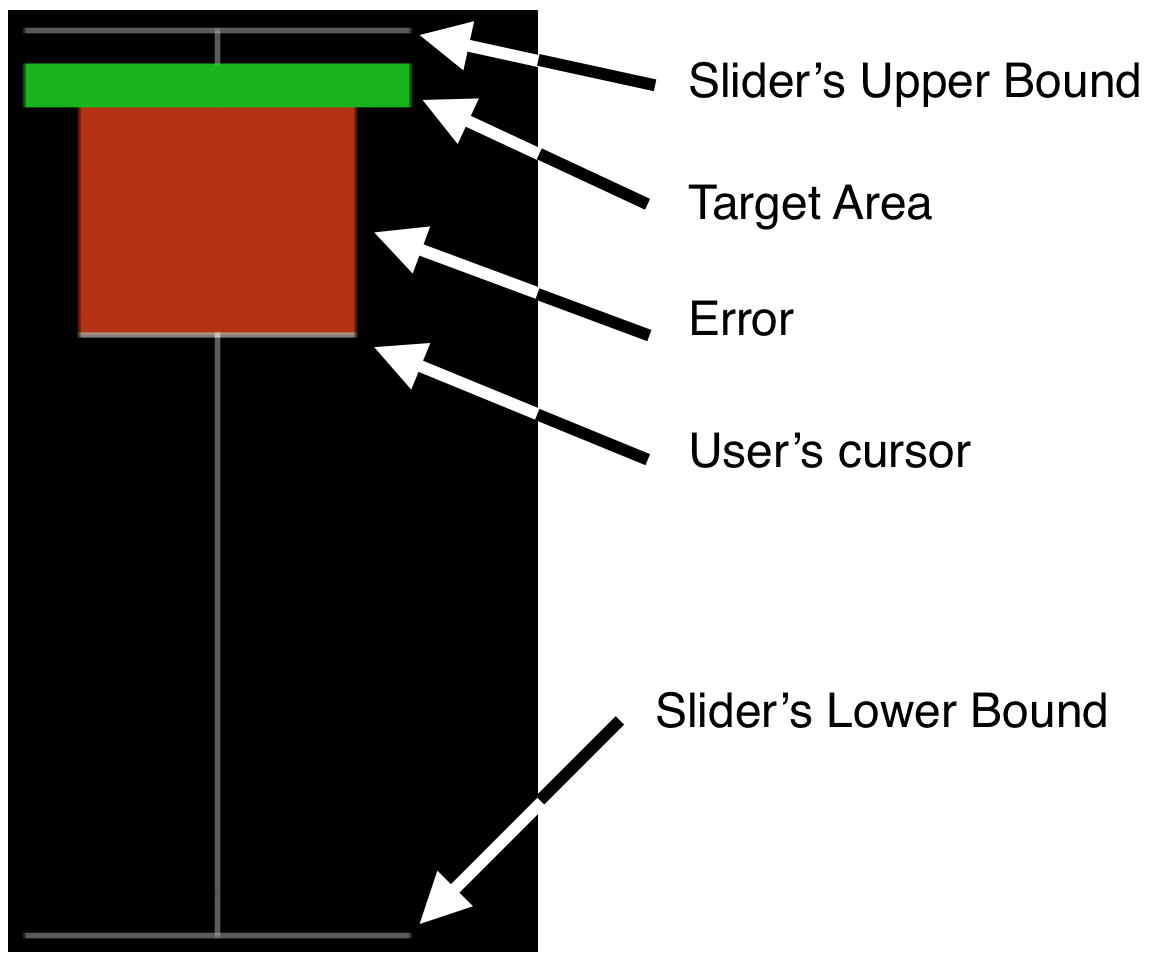
\includegraphics[width=0.7\columnwidth]{figures/slidertask}
  \caption{}
  \label{fig:slidertask}
\end{figure}
%================================================

Participants were asked to be as fast and accurate as possible on the pointing task. As in \cite{Buck:Motor}, the error rate is forced to zero, meaning that the task must be finished successfully; this happens when the user’s cursor enters the target area. To avoid additional actions to confirm the pointing, a time lapse of 1 second is used as in \cite{Zhang:2012:MDE:2212776.2223704}; after this, a new target area appears in a predefined distance of 60mm/270px in relation to the user’s cursor.

The target’s width and distance were selected in order to keep a single Fitt’s index of difficulty  (ID) of 4, resembling the ID used in \cite{Buck:Motor}; this value was given by $ID = log2((D/W)+1)$, where \textit{D} is the distance between the user’s cursor position and the target area, and \textit{W} is the target area width. The Control-Display gain difference for both large sliders (CD gain = 1,83) and small sliders (CD gain = 0,52) are within the range of the CD gains that do not affect the movement time as computed in \cite{Buck:Motor}.

%----------------------------------------------------------------------------------------
\subsection{Procedure}
%----------------------------------------------------------------------------------------
At first, participants were introduced to the prototypes and tasks through a training phase; after this, the trials started. As in \cite{Grossman:2005:BCE:1054972.1055012}, the tasks were performed in pseudo-random order through 2 blocks (according to the Interaction Technique variable) to avoid disturbing the participants with several changes among the grasping conditions. Half of the participants started with the One-handed condition and the other half with the Two-handed condition. Each block was divided in 4 sub-blocks representing the 4 possible combinations from the Length $\times$ Orientation conditions which were presented to the participants in random order; a small break was given to participants after each sub-block. For each sub-block 17 repetitions were performed; the first repetition was used for training. A total of 1536 pointing tasks were collected, by 12 participants $\times$ 16 task repetitions $\times$ 2 Interaction Techniques $\times$ 2 Lengths $\times$ 2 Orientations (192 measures for each Interaction Technique $\times$ Length $\times$ Orientation conditions).

Along the experiment participants were recorded in order to analyse the way how they interacted with the prototypes when performing two-handed interaction. The study ended with participants answering a SUS form to evaluate the 8 presented conditions (2 Interaction Techniques $\times$ 2 Lengths $\times$ 2 Orientations).
%================================================
%\begin{figure*}
%  \centering
%  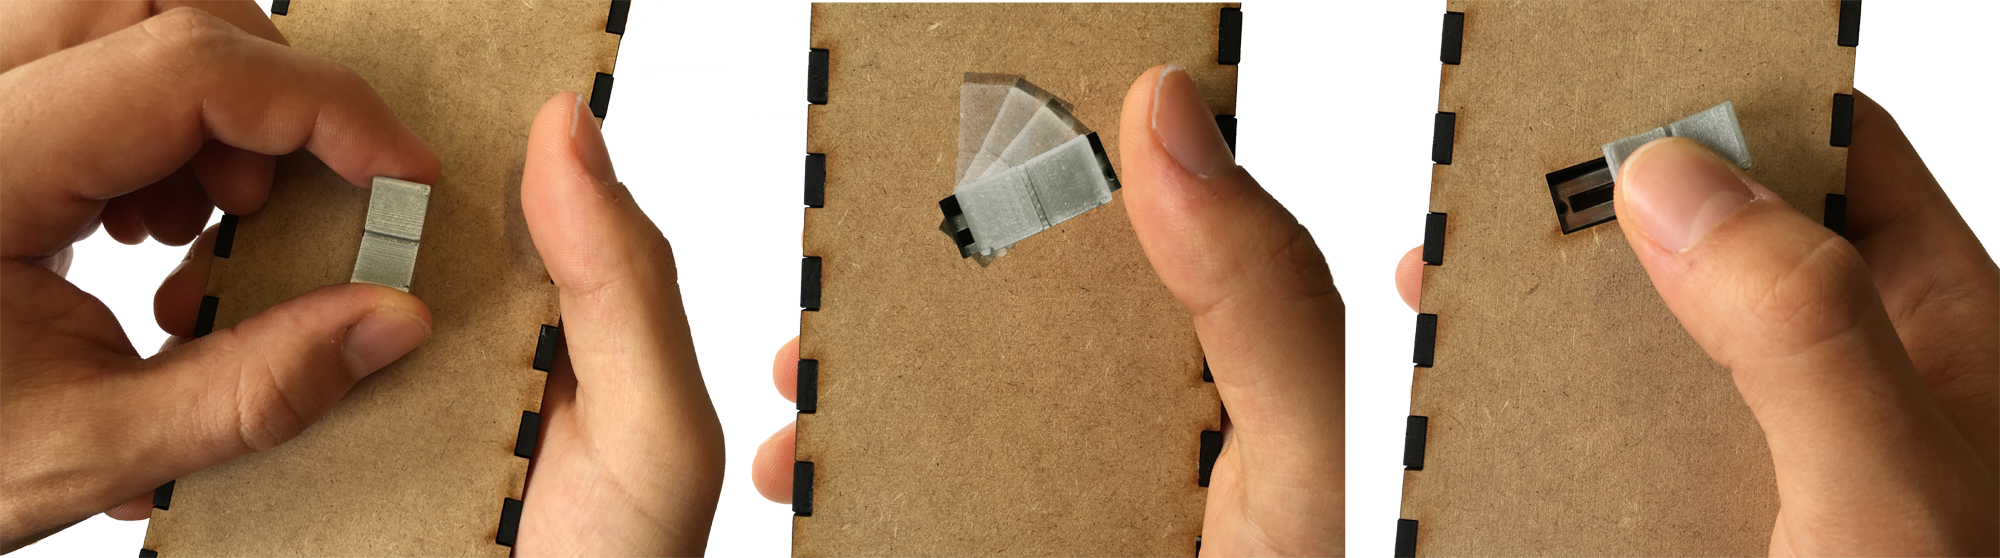
\includegraphics[width=1.7\columnwidth]{figures/portada}
%  \caption{Exemple de figure sur deux colonnes. Les figures sur deux colonnes doivent \^etre plac\'ee en haut ou en bas de page. Utilisez des images haute-r\'esolution, 300+ dpi, lisible une fois imprim\'ees, que ce soit en couleur ou en noir et blanc. Image: \ccbynd~ayman on
%    Flickr.}~\label{fig:portada}
%\end{figure*}
%================================================ 


%================================================
%\begin{table}
%  \centering
%  \begin{tabular}{l r r r}
    % \toprule
%    & & \multicolumn{2}{c}{\small{\textbf{Les conditions exp\'erimentales}}} \\
%    \cmidrule(r){3-4}
%    {\small\textit{Nom}}
%    & {\small \textit{Premier}}
%      & {\small \textit{Deuxi\`eme}}
%    & {\small \textit{Final}} \\
%    \midrule
%    Marsden & 223.0 & 44 & 432,321 \\
%    Nass & 22.2 & 16 & 234,333 \\
%    Borriello & 22.9 & 11 & 93,123 \\
%   Karat & 34.9 & 2200 & 103,322 \\
    % \bottomrule
%  \end{tabular}
%  \caption{Les l\'egendes des tableaux sont plac\'ees sous ceux. Nous recommandons l'utilisation de lignes de 1 point, 25\% noir. Limitez l'utilisation des lignes inutiles.}~\label{tab:table1}
%\end{table}
%================================================

%----------------------------------------------------------------------------------------
\section{Future Work}
%----------------------------------------------------------------------------------------
Thinking about the deformation factor we aim to apply this to particular areas of a tangible slider  such as the slider’s knob instead of affecting the whole widget as it is done when the orientation is changed. Indeed, sliders’ knobs can offer different affordance according to the interaction technique applied to it and thus, could affect the performance of a task.
%----------------------------------------------------------------------------------------
\section{Remerciements}
%----------------------------------------------------------------------------------------
Ce document est bas\'e sur le mod\`ele des soumissions aux conf\'erences SIGCHI, ainsi que sur ceux des conf\'erences IHM pr\'ec\'edentes. Merci \`a leurs nombreux auteurs.

% Balancing columns in a ref list is a bit of a pain because you
% either use a hack like flushend or balance, or manually insert
% a column break.  http://www.tex.ac.uk/cgi-bin/texfaq2html?label=balance
% multicols doesn't work because we're already in two-column mode,
% and flushend isn't awesome, so I choose balance.  See this
% for more info: http://cs.brown.edu/system/software/latex/doc/balance.pdf
%
% Note that in a perfect world balance wants to be in the first
% column of the last page.
%
% If balance doesn't work for you, you can remove that and
% hard-code a column break into the bbl file right before you
% submit:
%
% http://stackoverflow.com/questions/2149854/how-to-manually-equalize-columns-
% in-an-ieee-paper-if-using-bibtex
%
% Or, just remove \balance and give up on balancing the last page.
%
\balance{}

% REFERENCES FORMAT
% References must be the same font size as other body text.
%\bibliographystyle{unsrt}
\bibliographystyle{SIGCHI-Reference-Format}
\bibliography{sample}

\end{document}
%----------------------------------------------------------------------------------------

%%% Local Variables:
%%% mode: latex
%%% TeX-master: t
%%% End:
